\section{Theorie}
\label{sec:Theorie}
\begin{wrapfigure}{R}{5cm}
  \centering
  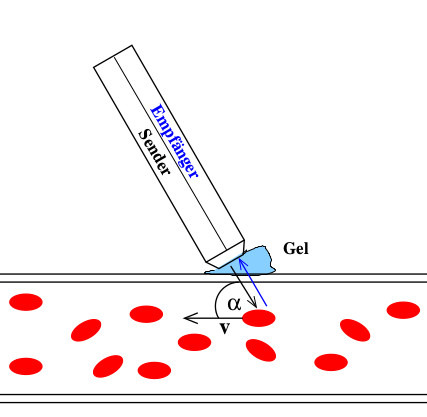
\includegraphics[width=0.35\textwidth]{Bilder/sonographie.png}
  \caption{Darstellung der Messmethode unter Verwendung des Impuls-Echo-Verfahrens. \cite{Anleitung}}
  \label{fig:doppler}
\end{wrapfigure}
Unter Ultraschall wird der Frequenzbereich oberhalb der Hörschwelle mit Frequenzen von $\SI{20}{\kilo\Hz}$ bis $\SI{1}{\giga\Hz}$ verstanden.
Die Ultraschall-Sonographie macht sich den Doppler-Effekt zur Untersuchung von Strömungen auf ihre charakteristischen Eigenschaften zunutze.\\
Unter dem \textbf{Doppler-Effekt} werden Änderungen der Frequenz, verursacht durch Relativbewegungen zwischen der Schallquelle und dem Empfänger, verstanden.
Es treten hierbei zwei verschiedene Fälle auf, da die Schallwelle an ein Übertragungsmedium gekoppelt ist.\\
Bewegt sich die Schallquelle, und der Schallempfänger ruht, so staucht/streckt die Bewegung der Schallquelle zwischen zwei Wellenbergen die Wellenlänge des ausgesendeten Schalls.
Die Frequenz, welche der ruhende Empfänger wahrnimmt, wird daher von der Ruhefrequenz $\nu_0$ (keine Relativbewegung zwischen Quelle und Empfänger) zu einer höheren Frequenz $\nu_\mathrm{kl}$ bzw. einer kleineren Frequenz $\nu_\mathrm{gr}$ verschoben:
\begin{equation}
  \label{eqn:doppleruno}
  \nu_\mathrm{kl/gr}=\frac{\nu_0}{1\mp \frac{v}{c}}\text{.}
\end{equation}
Bewegt sich stattdessen der Empfänger bei ruhender Quelle, so ändert sich die Wellenlänge nicht. Der Empfänger nimmt sie nur verkürzt/verlängert wahr, da er sich relativ zur Ausbreitung der Schallwelle bewegt.
Der Empfänger nimmt die höhere Frequenz $\nu_\mathrm{h}$ bzw. die geringere Frequenz $\nu_\mathrm{n}$ wahr:
\begin{equation}
  \label{eqn:dopplerzwo}
  \nu_\mathrm{h/n}=\nu_0 \left(1\pm\frac{v}{c}\right)\text{.}
\end{equation}

In der Doppler-Sonographie wird das Impuls-Echo-Verfahren verwendet, Empfänger und Sender befinden sich also am gleichen Ort.\\
Wie in Abbildung \ref{fig:doppler} dargestellt, dient zunächst die Ultraschallsonde als Sender und die in rot dargestellten Blutkörperchen bewegen sich als Empfänger bezüglich der Schallquelle(vgl. Formel \eqref{eqn:dopplerzwo}). Die Schallwelle wird an den roten Blutkörperchen reflektiert, sodass die Blutkörperchen zur Signalquelle werden und sich bezüglich des ruhenden Empfängers bewegen(vgl. Formel \eqref{eqn:doppleruno}).
Für die Verschiebung der Frequenz der Ultraschallwelle bezüglich $\nu_0$ ergibt sich:
\begin{equation}
  \label{eqn:verschiebung}
  \Delta \nu=2\cdot\nu_0\frac{v}{c}\cos{\alpha} \text{.}
\end{equation}
Hierbei ist $v$ die Geschwindigkeit des Objekts (im Beispiel: das rote Blutkörperchen) und $c$ die Schallgeschwindigkeit.
Der Winkel $\alpha$ ist der Winkel zwischen der Geschwindigkeit $\vec{v}$ und der Wellennormalen der ein-und auslaufenden Welle.

Ultraschallwellen können auf unterschiedliche Arten erzeugt werden. Im vorliegenden Fall wird der reziproke \textbf{piezo-elektrische Effekt} verwendet.
Wird ein piezoelektrischer Kristall in ein elektrisches Wechselfeld gebracht, so entsteht aufgrund der Deformation des Kristalls eine elektrischen Spannung an dessen Oberfläche. Durch das elektrischen Wechselfelds,lassen sich, wenn eine polare Achse des Kristalls in Richtung des elektrischen Felds ausgerichtet ist, also Schwingungen anregen.
Beim Schwingen strahlt der piezoelektrische Kristall Ultraschallwellen ab.\\
Der Kristall kann ebenso als Empfänger dienen, auftreffende Schallwellen regen diesen hierbei zum Schwingen an.
%Eventuell noch Formel zur Berechnung des Dopplerwinkels
